\documentclass{article}
\usepackage{amsmath,amssymb}
\usepackage{graphicx}
\usepackage{enumerate}
\usepackage{hyperref}
\usepackage{subcaption}
\usepackage{caption}
\usepackage{xcolor}
\usepackage{float}

\pagestyle{empty} \addtolength{\textwidth}{1.0in}
\addtolength{\textheight}{0.5in}
\addtolength{\oddsidemargin}{-0.5in}
\addtolength{\evensidemargin}{-0.5in}
\newcommand{\ruleskip}{\bigskip\hrule\bigskip}
\newcommand{\nodify}[1]{{\sc #1}}
\newcommand{\points}[1]{{\textbf{[#1 points]}}}
\newcommand{\subquestionpoints}[1]{{[#1 points]}}
\newenvironment{answer}{{\bf Answer:} \sf }{}%

\newcommand{\bitem}{\begin{list}{$\bullet$}%
{\setlength{\itemsep}{0pt}\setlength{\topsep}{0pt}%
\setlength{\rightmargin}{0pt}}}
\newcommand{\eitem}{\end{list}}

\setlength{\parindent}{0pt} \setlength{\parskip}{0.5ex}
\setlength{\unitlength}{1cm}

\newcommand{\pa}[1]{[[PA: #1]]}

\renewcommand{\Re}{{\mathbb R}}
\newcommand{\E}{{\rm E}}
\begin{document}

\pagestyle{myheadings} \markboth{}{CS 294-158 Deep Unsupervised Learning, Homework 2, Spring 2020}

{\huge
\noindent Homework 2: Flow Models}
\ruleskip

{\bf Deliverable}: This PDF write-up by {\bf Tuesday February 25th, 23:59pm}.  Your PDF should be generated by simply replacing the placeholder images of this LaTeX document with the appropriate solution images that will be generated automatically when solving each question. The solution images are automatically generated and saved using the accompanying IPython notebook. Your PDF is to be submitted into Gradescope. This PDF already contains a few solution images.  These images will allow you to check your own solution to ensure correctness.


\vspace{.2in}

%--------------------------------------------------------------------------------
%--------------------------------------------------------------------------------
%--------------------------------------------------------------------------------
\noindent {\bf Question 1: 2D Data}
%--------------------------------------------------------------------------------
%--------------------------------------------------------------------------------
%--------------------------------------------------------------------------------

\begin{enumerate}[(a)]

\item {\bf [15pt] Autoregressive Flow} \\\\
Final test loss for dataset 1: 1.3092 nats / dim
\begin{figure}[H]
    \centering
    \begin{subfigure}{0.32\textwidth}
        \centering
        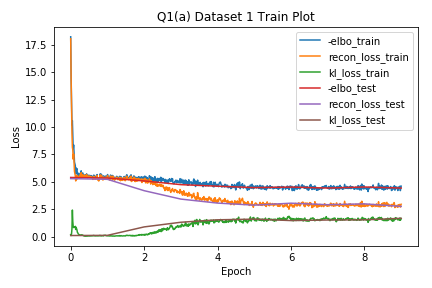
\includegraphics[width=\textwidth]{figures/q1_a_dset1_train_plot.png}
        \caption{Training curve}
    \end{subfigure}
    \begin{subfigure}{0.32\textwidth}
        \centering
        \includegraphics[width=\textwidth]{figures/q1_a_dset1_densities.png}
        \caption{Learned distribution}
    \end{subfigure}
    \begin{subfigure}{0.32\textwidth}
        \centering
        \includegraphics[width=\textwidth]{figures/q1_a_dset1_latents.png}
        \caption{Latent Space}
    \end{subfigure}
    \caption{Results for Dataset 1}
\end{figure}
Final test loss for dataset 2: 0.0000  nats / dim
\begin{figure}[H]
    \centering
    \begin{subfigure}{0.32\textwidth}
        \centering
        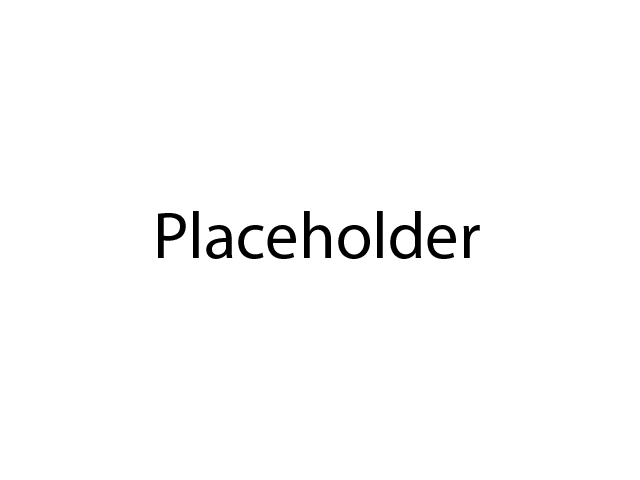
\includegraphics[width=\textwidth]{figures/q1_a_dset2_train_plot.png}
        \caption{Training curve}
    \end{subfigure}
    \begin{subfigure}{0.32\textwidth}
        \centering
        \includegraphics[width=\textwidth]{figures/q1_a_dset2_densities.png}
        \caption{Learned distribution}
    \end{subfigure}
    \begin{subfigure}{0.32\textwidth}
        \centering
        \includegraphics[width=\textwidth]{figures/q1_a_dset2_latents.png}
        \caption{Latent Space}
    \end{subfigure}
    \caption{Results for Dataset 2}
\end{figure}

\newpage

\item {\bf [15pt] RealNVP} \\\\
Final test loss for dataset 1: 2.0586  nats / dim
\begin{figure}[H]
    \centering
    \begin{subfigure}{0.32\textwidth}
        \centering
        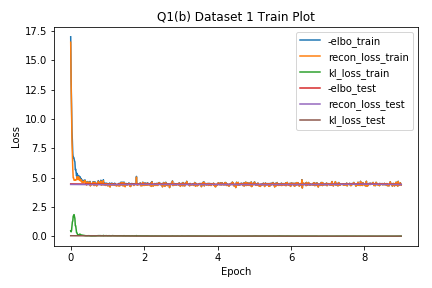
\includegraphics[width=\textwidth]{figures/q1_b_dset1_train_plot.png}
        \caption{Training curve}
    \end{subfigure}
    \begin{subfigure}{0.32\textwidth}
        \centering
        \includegraphics[width=\textwidth]{figures/q1_b_dset1_densities.png}
        \caption{Learned distribution}
    \end{subfigure}
    \begin{subfigure}{0.32\textwidth}
        \centering
        \includegraphics[width=\textwidth]{figures/q1_b_dset1_latents.png}
        \caption{Latent Space}
    \end{subfigure}
    \caption{Results for Dataset 1}
\end{figure}
Final test loss for dataset 2: 0.0000  nats / dim
\begin{figure}[H]
    \centering
    \begin{subfigure}{0.32\textwidth}
        \centering
        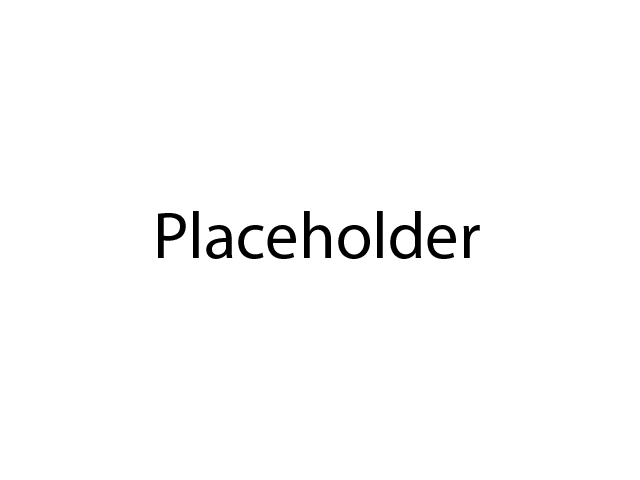
\includegraphics[width=\textwidth]{figures/q1_b_dset2_train_plot.png}
        \caption{Training curve}
    \end{subfigure}
    \begin{subfigure}{0.32\textwidth}
        \centering
        \includegraphics[width=\textwidth]{figures/q1_b_dset2_densities.png}
        \caption{Learned distribution}
    \end{subfigure}
    \begin{subfigure}{0.32\textwidth}
        \centering
        \includegraphics[width=\textwidth]{figures/q1_b_dset2_latents.png}
        \caption{Latent Space}
    \end{subfigure}
    \caption{Results for Dataset 2}
\end{figure}
\end{enumerate}



%--------------------------------------------------------------------------------
%--------------------------------------------------------------------------------
%--------------------------------------------------------------------------------
\newpage
\noindent {\bf Question 2: Autoregressive Flows for Images [20pt]}
%--------------------------------------------------------------------------------
%--------------------------------------------------------------------------------
%--------------------------------------------------------------------------------


\\\\

Final test loss: 0.2258  nats / dim
\begin{figure}[H]
    \centering
    \begin{subfigure}{0.45\textwidth}
        \centering
        \includegraphics[width=\textwidth]{figures/q2_train_plot.png}
        \caption{Training curve}
    \end{subfigure}
    \\
    \begin{subfigure}{0.48\textwidth}
        \centering
        \includegraphics[width=\textwidth]{figures/q2_samples.png}
        \caption{Samples}
    \end{subfigure}
    \begin{subfigure}{0.48\textwidth}
        \centering
        \includegraphics[width=\textwidth]{figures/q2_flooredsamples.png}
        \caption{Samples, removing noise from dequantization}
    \end{subfigure}
\end{figure}

%--------------------------------------------------------------------------------
%--------------------------------------------------------------------------------
%--------------------------------------------------------------------------------
\newpage
\noindent {\bf Question 3: RealNVP on Higher Dimensions}
%--------------------------------------------------------------------------------
%--------------------------------------------------------------------------------
%--------------------------------------------------------------------------------

\begin{enumerate}[(a)]
\item {\bf [40pt] RealNVP} \\\\
Final test loss: 0.55  bits / dim
\begin{figure}[H]
    \centering
    \begin{subfigure}{0.45\textwidth}
        \centering
        \includegraphics[width=\textwidth]{figures/q3_a_train_plot.png}
        \caption{Training curve}
    \end{subfigure}
    \\
    \begin{subfigure}{0.48\textwidth}
        \centering
        \includegraphics[width=\textwidth]{figures/q3_a_samples.png}
        \caption{Samples}
    \end{subfigure}
    \begin{subfigure}{0.48\textwidth}
        \centering
        \includegraphics[width=\textwidth]{figures/q3_a_interpolations.png}
        \caption{Interpolations}
    \end{subfigure}
\end{figure}
\newpage

\item {\bf [10pt] Bad Masking} \\\\
Final test loss: 0.0000  nats / dim
\begin{figure}[H]
    \centering
    \begin{subfigure}{0.45\textwidth}
        \centering
        \includegraphics[width=\textwidth]{figures/q3_b_train_plot.png}
        \caption{Training curve}
    \end{subfigure}
    \\
    \begin{subfigure}{0.48\textwidth}
        \centering
        \includegraphics[width=\textwidth]{figures/q3_b_samples.png}
        \caption{Samples}
    \end{subfigure}
    \begin{subfigure}{0.48\textwidth}
        \centering
        \includegraphics[width=\textwidth]{figures/q3_b_interpolations.png}
        \caption{Interpolations}
    \end{subfigure}
\end{figure}
\end{enumerate}

\newpage
\noindent {\bf Bonus Questions (Optional)}
\begin{enumerate}

\item {\bf [10pt] Multiscale RealNVP} \\\\
Final test loss: 0.0000  nats / dim
\begin{figure}[H]
    \centering
    \begin{subfigure}{0.45\textwidth}
        \centering
        \includegraphics[width=\textwidth]{figures/q3_bonus_a_train_plot.png}
        \caption{Training curve}
    \end{subfigure}
    \\
    \begin{subfigure}{0.48\textwidth}
        \centering
        \includegraphics[width=\textwidth]{figures/q3_bonus_a_samples.png}
        \caption{Samples}
    \end{subfigure}
    \begin{subfigure}{0.48\textwidth}
        \centering
        \includegraphics[width=\textwidth]{figures/q3_bonus_a_interpolations.png}
        \caption{Interpolations}
    \end{subfigure}
\end{figure}

\newpage
\item {\bf [5pt] Glow} \\\\
Final test loss: 0.0000  nats / dim
\begin{figure}[H]
    \centering
    \begin{subfigure}{0.45\textwidth}
        \centering
        \includegraphics[width=\textwidth]{figures/q3_bonus_b_train_plot.png}
        \caption{Training curve}
    \end{subfigure}
    \\
    \begin{subfigure}{0.48\textwidth}
        \centering
        \includegraphics[width=\textwidth]{figures/q3_bonus_b_samples.png}
        \caption{Samples}
    \end{subfigure}
    \begin{subfigure}{0.48\textwidth}
        \centering
        \includegraphics[width=\textwidth]{figures/q3_bonus_b_interpolations.png}
        \caption{Interpolations}
    \end{subfigure}
\end{figure}
\end{enumerate}

\end{document}